\renewcommand{\theequation}{\theenumi}
\renewcommand{\thefigure}{\theenumi}
\renewcommand{\thetable}{\theenumi}
\begin{enumerate}[label=\thesection.\arabic*.,ref=\thesection.\theenumi]
\numberwithin{equation}{enumi}
\numberwithin{figure}{enumi}
\numberwithin{table}{enumi}

\item A fair coin is tossed 10 times. What is the probability that ONLY the first two tosses will yield heads?
\begin{enumerate}
\begin{multicols}{2}
\setlength\itemsep{1em}
{\small
\item $
\brak{\frac{1}{2}}^2
$
\item $
{\comb{10}{2}}\brak{\frac{1}{2}}^2
$
\item $
\brak{\frac{1}{2}}^{10}
$
\item $
{\comb{10}{2}}\brak{\frac{1}{2}}^{10}
$
}
\end{multicols}
\end{enumerate}
%
\solution
Let $M \sim B\brak{n,h}$ be a random variable representing number of 'heads' in 10 tosses.
So M has a binomial distribution :
\begin{align}
    \pr{M=k} = \comb{n}{k} \times (h)^{n-k} \times (t)^{k}\label{0.0.1}
\end{align}
Where
\begin{itemize}
    \item n = Total number of tosses = 10
    \item h = Probability that 'head' appears in a toss = \( \frac{1}{2} \)
    \item t = Probability that 'tail' appears in a toss = \( \frac{1}{2} \)
\end{itemize}
\bigskip
So,
\begin{align}
    \pr{M=k} = \comb{10}{k} \times \brak{\frac{1}{2}}^{10-k} \times \brak{\frac{1}{2}}^{k}\label{0.0.2}
\end{align}
\begin{table}[!ht]
    \begin{center}
        \small
        \resizebox{\columnwidth}{!}
        {
            \begin{tabular}{|c|c|}
                \hline
                n            & 10                                                                            \\
                \hline
                $\pr{M = 2}$ & $\comb{10}{2} \times \brak{\frac{1}{2}}^{10-2} \times \brak{\frac{1}{2}}^{2}$ \\
                \hline
                Calculation  & $\comb{10}{2} \times \brak{\frac{1}{2}}^{10}$                                 \\
                \hline
                Value        & 0.043945                                                                      \\
                \hline
            \end{tabular}
        }
    \end{center}
\end{table}
\begin{itemize}
    \item Number of ways of choosing 2 positions from 10 tosses = $\comb{10}{2}$
          \bigskip
    \item Number of favourable outcome = 1 (Choosing FIRST and SECOND tosses as heads)
          \bigskip
    \item Probability that chosen 2 'heads' are from FIRST and SECOND tosses = \(\displaystyle \frac{1}{\comb{10}{2}}\)
          \bigskip
\end{itemize}
Probability that ONLY the first 2 tosses yield heads
\begin{align}
    = & \pr{M = 2} \times \displaystyle \frac{1}{\comb{10}{2}}                    \\
    = & \comb{10}{2} \times \brak{\frac{1}{2}}^{10} \times \frac{1}{\comb{10}{2}} \\
    = & \brak{\frac{1}{2}}^{10}
\end{align}
%
\item Let the random variable X represent the number of times a fair coin needs to be tossed till two consecutive heads appear for the first time. The expectation of X is......

\item Let $X\in[0,1]$ and $Y\in[0,1]$ be two independent binary random variables. If $P(X=0) = p$ and $P(Y=0) = q$, then $P(X+Y\geqslant1)$ is equal to

\begin{enumerate}
\begin{multicols}{2}
\setlength\itemsep{1em}
{\small
\item $
pq + (1-p)(1-q)
$
\item pq
\item $p(1-q)$
\item $1-pq$
}
\end{multicols}
\end{enumerate}
%
\solution

Let $X \in \{0,1\}$ be the random variable, where X=0 represents that we get sum to be 8 or 9 and X=1 represents that we get sum between 2 and 12 except 8 and 9.\\
Total number of possible outcomes is :
\begin{equation}
    N = {\comb{6}{1}}\times{\comb{6}{1}} = 36
\end{equation}
 
Probability that the sum is neither 8 or 9 
\begin{equation}\label{me2005-38:eq:2}
  \pr{X=1} = 1-\pr{X=0}
\end{equation}
 Only 9 outcomes are favourable to the occurrence of X=0 .\\
Probability of getting sum 8 or 9 is :
\begin{equation}
    \pr{X=0} = \frac{9}{36}
             = \frac{1}{4}
\end{equation}
Substituting value in \eqref{me2005-38:eq:2} , we get
\begin{equation}
 \pr{X=1} = 1- \frac{1}{4}
          = \frac{3}{4}   
\end{equation}
Hence, the correct option is (d) \large$\frac{3}{4}$
\item A fair coin is tossed three times in succession. If the first toss produces a head, then the probability of getting exactly two heads in three tosses is:

\begin{enumerate}
\begin{multicols}{2}
\setlength\itemsep{1em}

\item $\frac{1}{8}$
\item $\frac{1}{2}$
\item $\frac{3}{8}$
\item $\frac{3}{4}$

\end{multicols}
\end{enumerate}

\item A player throws a ball at a basket kept at a distance. The probability that the ball falls into the basket in a single attempt is 0.1. The player attempts to throw the ball twice. Considering each attempt to be independent, the probability that this player puts the ball into the basket only in the second attempt is.........
\\
\solution
Let $X\in\mathbb{N}$ represent the number of times the experiment is performed. \\
$X=k$ represents $k-1$ failures were obtained before getting 1 success. $p$ represents the probability of success
\begin{align}
	p_X(k) &=
\begin{cases}
\brak{1-p}^{k-1}\times p & k\in \mathbb{N}\\
0 &  otherwise 
\end{cases}
\label{2020:eq:final_result}
\end{align}
Using \eqref{2020:eq:final_result} we get
\begin{align}
\pr{X=2}&=\brak{1-p}^{k-1}\times p\nonumber\\
&=\brak{0.9}\times 0.1=0.09
\end{align}

\item Shaquille O’ Neal is a 60\% career free throw shooter, meaning that he successfully makes 60 free throws out of 100 attempts on average. What is the probability that he will successfully make exactly 6 free throws in 10 attempts?
\begin{enumerate} [label={\Alph*)}]
\item 0.2508
\item 0.2816
\item 0.2934
\item 0.6000
\end{enumerate}
%
\solution
Let 
\begin{align}
X_{i}\in \{0,1\}
\end{align}
represent the $i^{th}$ free throw, where 1 represents a successful free throw attempt and 0 represents an unsuccessful attempt.
Let
\begin{align}
X=\sum_{i=1}^{n} X_{i}   
\end{align}
where n is the total number of free throws. Then, X has a binomial distribution with
\begin{align}
\pr {X=k}=\comb{n}{k} p^{k} q^{n-k}
\end{align}
Where,
\begin{align}
  &p=\frac{6}{10}\\
  &q=1-p=\frac{4}{10}\\
  &n=10
\end{align}
from the given information. Then,
\begin{align}
\pr{X=6}&=\comb{10}{6}\brak{\frac{6}{10}}^{6}\brak{\frac{4}{10}}^{4}
\end{align}
On simplifying we get,
\begin{align}
\pr{X=6}&=0.2508
\end{align}
Therefore, the probability that he will successfully make exactly 6 free throws in 10 attempts is 0.2508 and hence option (A) is correct.

%
\item  Consider a sequence of tossing a fair coin where outcomes of tosses are independent.The probability of getting the head for the third time in the fifth toss is
    \begin{enumerate}[label=(\Alph*)]
      \item $\dfrac{5}{16}$  \item $\dfrac{3}{16}$ \item $\dfrac{3}{5}$ \item $\dfrac{9}{16}$
    \end{enumerate}
    \solution
Let the random variable $X \in \{0,1\}$ denotes head and tail in a toss.As both are equally probable.
\begin{align}
    \pr{X=0}=\dfrac{1}{2}\\
    \pr{X=1}=\dfrac{1}{2}
\end{align}

\begin{table}[h]
\begin{tabular}{|c|c|}
\hline
\textbf{Event} & \textbf{Description}                 \\ \hline
A              & nth toss is a head                   \\ \hline
B              & Exactly k-1 heads in first four tosses \\ \hline
C              & nth toss is the third head           \\ \hline
\end{tabular}
\caption{Description of events used in problem}
\label{tab:Events}
\end{table}

\begin{align}
\pr{A}&=\pr{X=1}=\dfrac{1}{2}\\
\pr{B}&=\dfrac{{}^{n-1}C_{k-1}}{2^{n-1}}
\end{align}

\begin{align}
    C&=AB\\
    \pr{C}&=\pr{AB}
\end{align}
As A and B are independent events.
\begin{align}
    \pr{C}&=\pr{A}\pr{B}\\
    &=\dfrac{1}{2}\times\dfrac{{}^{n-1}C_{k-1}}{2^{n-1}}\\
    &=\dfrac{{}^{n-1}C_{k-1}}{2^n}
\end{align}
Here n=5,k=3
\begin{align}
    \pr{C|n=5,k=2}&=\dfrac{{}^{4}C_{2}}{2^{5}}\\
    &=\dfrac{6}{32}
\end{align}

Therefore probability of getting the head for the third time in the fifth toss is $\dfrac{3}{16}$. 


\item A box has ten light bulbs out of which two are defective, Two light bulbs are drawn from this box one after the other without replacement. The probability that both light bulbs drawn are not defective is 
\begin{enumerate}[label={\Alph*)}]
\begin{multicols}{4}
\setlength\itemsep{2em}
\item $\dfrac{8}{45}$
\item $\dfrac{28}{45}$
\item $\dfrac{16}{25}$
\item $\dfrac{4}{5}$
\end{multicols}
\end{enumerate}
\solution
Let $X_i \in \cbrak{0,1}$ represent the $i^{th}$ draw, where 0 denotes a defective bulb and 1 denotes a non-defective bulb.
\begin{table}[h]
\centering 
\caption{}
\begin{tabular}{|c|c|c|}
\hline
           & $X_1 = 0$ & $X_1 = 1$\\
\hline
$X_2 = 0$  & 2/90      & 16/90  \\
\hline
$X_2 = 1$  & 16/90      & 56/90  \\
\hline
\end{tabular}
\label{xe2015:table}
\end{table}
 
Table \ref{table} represents the probabilities of all possible cases when two bulbs are drawn one by one without replacement.
Probability that both of the bulbs are non-defective (by substituting values from table \ref{table})
\begin{align}
    &= \Pr\brak{X_2 = 1|X_1 = 1}\Pr\brak{X_1 = 1}\\
    &= \dfrac{56}{90}\\
    &= \dfrac{28}{45}
\end{align}
So the correct option is (B)

\item Three fair dies are rolled simultaneously. The probability of getting a sum of 5 is
\begin{enumerate}
    \item $\frac{1}{108}$
    \item $\frac{1}{72}$
    \item $\frac{1}{54}$
    \item $\frac{1}{36}$
\end{enumerate}
%
\solution


Let
$X_i\in\,$\cbrak{1,2,3,4,5,6}, i = 1,2,3, be the random variables representing the outcome for each die. As the dies are fair, the probability mass function (pmf) is expressed as
\begin{align}
    p_{X_i}(n) = \pr{X_i = n} = 
\begin{cases}
\frac{1}{6} & 1 \le n \le 6
\\
0 & otherwise
\end{cases}\label{1}
\end{align}
Let X be a random variable denotes the desired outcome,
\begin{align}
    X=X_1+X_2+X_3\label{2}\\
    \implies X\in\cbrak{3,4,\cdots,18}
\end{align}

We have to find $P_X(n)$ = $\pr{X_1+X_2+X_3=n}$
\begin{multline}
    p_X(n)=\pr{X_1+X_2+X_3=n}\\
   =\pr{X_1+X_2=n-X_3}\\
    =\Sigma_{k}{\pr{X_1+X_2=n-k|X_3=k}p_{X_3}(k)}\label{3}
\end{multline}
As $X_1,X_2,X_3$ are independent, After unconditioning
\begin{align}
    \pr{X_1+X_2=n-k|X_3=k}=\pr{X_1+X_2=n-k}\label{6}
\end{align}
Using \eqref{6} in \eqref{3}
\begin{multline}
    p_X(n)=\Sigma_{k}{\pr{X_1+X_2=n-k|X_3=k}p_{X_3}(k)}\\
    =\Sigma_{k}{\pr{X_1+X_2=n-k}p_{X_3}(k)}\\
    =\Sigma_{k}{\brak{\Sigma_{a}{\pr{X_1=n-k-a|X_2=a}\pr{X_2=a}}}p_{X_3}(k)}\\
    =\Sigma_{k}{\brak{\Sigma_{a}{\pr{X_1=n-k-a}\pr{X_2=a}}}p_{X_3}(k)}\\
    =\Sigma_{k}{\brak{\Sigma_{a}{p_{X_1}\brak{n-k-a}p_{X_2}\brak{a}}}p_{X_3}(k)}\label{4}
\end{multline}
Equation \eqref{4} can be written as follows using convolution operation,
\begin{align}
    \nonumber p_X(n)&=\Sigma_{k}{\brak{\Sigma_{a}{p_{X_1}\brak{n-k-a}p_{X_2}\brak{a}}}p_{X_3}(k)}\\
    &=p_{X_1}\brak{n}*p_{X_2}\brak{n}*p_{X_3}\brak{n}\label{5}
\end{align}
The Z-transform of $p_X(n)$ is defined as
\begin{align}
P_X(z) = \sum_{n = -\infty}^{\infty}p_X(n)z^{-n}, \quad z \in \mathbb{C}
\label{7}
\end{align}
%
From \eqref{1} and \eqref{7}, 
\begin{align}
\nonumber P_{X_1}(z) =P_{X_2}(z)&=P_{X_3}(z)\\
&= \frac{1}{6}\sum_{n = 1}^{6}z^{-n}
\\
&=\frac{z^{-1}\brak{1-z^{-6}}}{6\brak{1-z^{-1}}}, \quad \abs{z} > 1
\label{8}
\end{align}
upon summing up the geometric progression. 
From \eqref{5},
\begin{align}
\because p_X(n) &= p_{X_1}(n)*p_{X_2}(n)*p_{X-3}(n),
\\
P_X(z) &= P_{X_1}(z) P_{X_2}(z)P_{X_3}(z)
\label{9}
\end{align}
The above property follows from Fourier analysis and is fundamental to signal processing.\\
From \eqref{8} and \eqref{9},
\begin{align}
    P_X{\brak{z}}&=\cbrak{\frac{z^{-1}\brak{1-z^{-6}}}{6\brak{1-z^{-1}}}}^3\\
    &= \frac{1}{216}\frac{z^{-3}\brak{1-3z^{-6}+3z^{-12}-z^{-18}}}{\brak{1-z^{-1}}^3}\label{10}
\end{align}
Using the fact that,
\begin{align}
p_X(n-k) &\system{Z}P_X(z)z^{-k},
\\
nu(n)&\system{Z} \frac{z^{-1}}{\brak{1-z^{-1}}^2}\\
n^2u(n)&\system{Z} \frac{z^{-1}\brak{1+z^{-1}}}{\brak{1-z^{-1}}^3}\\
(n^2+n)u(n)&\system{Z} \frac{2z^{-1}}{\brak{1-z^{-1}}^2}
\end{align}
after some algebra, it can be shown that,
\begin{multline}
\frac{1}{216\times 2}\lsbrak{\brak{(n-2)^2+n-2}u(n-2)} \\-3 \brak{(n-8)^2+n-8}u(n-8)\\+3\brak{(n-14)^2+n-14}u(n-14)\\-\rsbrak{\brak{(n-20)^2+n-20}u(n-20)}
\\
\system{Z}
\frac{1}{216}\frac{z^{-3}\brak{1-3z^{-6}+3z^{-12}-z^{-18}}}{\brak{1-z^{-1}}^3}
\label{11}
\end{multline}
where 
\begin{align}
u(n) =
\begin{cases}
1 & n \ge 0
\\
0 & n < 0\label{13}
\end{cases}
\end{align}
From \eqref{7},\eqref{10} and \eqref{11},
\begin{multline}
p_{X}(n) = \frac{1}{216\times 2}\lsbrak{\brak{(n-2)^2+n-2}u(n-2)} \\-3 \brak{(n-8)^2+n-8}u(n-8)\\+3\brak{(n-14)^2+n-14}u(n-14)\\-\rsbrak{\brak{(n-20)^2+n-20}u(n-20)}
\label{12}
\end{multline}
From \eqref{13} and \eqref{12},
\begin{align}
p_X(n) &= 
\begin{cases}
0 & n < 3\\
\frac{n^2-3n+2}{432} &  3 \le n \le  8\\
\frac{42n-2n^2-166}{432} & 8 < n \le 14\\
\frac{n^2-39n+380}{432} & 14 < n \le 18\\
0 & n > 18\label{14}
\end{cases}
\end{align}
\begin{figure}[htp]
    \centering
    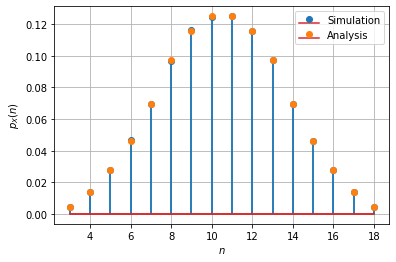
\includegraphics[width=\columnwidth]{solutions/xe/2017/figures/assign3_stem.png}
    \caption{Probability mass function of X}{ (simulations are close to analysis)}
\end{figure}
We need probability of getting sum of 5,\\$\implies$ n=5 \\from \eqref{14} and using n=5,
\begin{align}
    p_X(5)&=\frac{5^2-3(5)+2}{432}\\
    p_X(5)&=\frac{12}{432}\\
    p_X(5)&=\frac{1}{36}
\end{align}

Therefore the probability of getting a sum of 5 when three fair dies are rolled is $\frac{1}{36}$.\\
\textbf{Ans: Option (D)}



%
\item The probability of a resistor being defective is 0.02. There are 50 such resistors in a circuit. The probability of two or more defective resistors in the circuit (round off to two decimal places) is ---
%
\solution
Consider, Probability of a defective resistor 
$= P   = 0.02 = \dfrac{1}{50}$. \\
Total number of resistors = n = 50. \\
Let X be number of defective resistors. \\
By Binomial distribution, \\
\begin{align}
Pr(X = k) = \binom{n}{k}\brak{P}^k\brak{1 - P}^{n-k} 
\end{align}
\begin{align}
Pr(X = 0) &= \binom{50}{0}\brak{\dfrac{1}{50}}^0\brak{1 - \dfrac{1}{50}}^{50-0} 
\end{align}
\begin{align}
\implies Pr(X = 0) &= \brak{\dfrac{49}{50}}^{50} 
\end{align}
\begin{align}
Pr(X = 1) &= \binom{50}{1}\brak{\dfrac{1}{50}}^1\brak{1 - \dfrac{1}{50}}^{50-1} 
\end{align}
\begin{align}
\implies Pr(X = 1) &= \brak{\dfrac{49}{50}}^{49}
\end{align}
\begin{align*}
\Pr{(X \ge 2)} &= 1 - \Pr{(X < 2)} \\
\Pr{(X \ge 2)} &= 1 - \brak{\Pr{(X = 0)} + \Pr{(X = 1)}} \\
\Pr{(X \ge 2)} &= 0.2642 
\end{align*}

%
\item For each element in a set of size 2n, an unbiased coin is tossed. The 2n coin tosses are independent. An element is chosen if the corresponding coin toss were head. The probability that exactly n elements are chosen is:\\
\begin{enumerate}
    \item $\frac{\comb{2n}{n}}{4^{n}}$ \hspace{1cm}\\
    \item $\frac{\comb{2n}{n}}{2^{n}}$ \hspace{1cm}\\
    \item $\frac{1}{\comb{2n}{n}}$ \hspace{1cm}\\
    \item $\frac{1}{2}$
\end{enumerate}
%
\solution

The number of elements chosen is equal to the number of heads obtained by 2n coin tosses.
Let X be a random variable with value of X equal to the number of heads obtained.\\
Probability of getting a head, $p=\frac{1}{2}$\\
Probability of getting a tail, $q=\frac{1}{2}$\\
Probability that n elements are chosen out of 2n elements is \pr{X=n}\\
From binomial distribution we know that,
\begin{align}
\pr{X=r}&=\comb{2n}{r}p^{r}q^{2n-r}\\
\pr{X=n}&=\comb{2n}{n} \times \brak{\frac{1}{2}}^{n}  \times \brak{\frac{1}{2}}^{n}\\
        &=\frac{\comb{2n}{n}}{4^{n}}
\end{align}
Hence option (A) is correct.


%
\item  In an industry, the probability of an accident occurring in a given month is $\frac{1}{100}$. Let $\pr{n}$ denote the probability that there will be no accident over a period of '$n$' months. Assume that the events of individual months are independent of each other. The smallest integer value of '$n$' such that $\pr{n}\le \frac{1}{2} $ is .............(\textit{round off to the nearest integer}).\\
%
\solution
Let A be the event of an accident occurring in a given month.
So, 
\begin{align}
    \pr{A}&=\frac{1}{100}\\
    \pr{A^{\prime}}&=1-\pr{A}\\
    \pr{A^{\prime}}&=\frac{99}{100}
\end{align}
So, $\pr{n}$ can be written as:
\begin{align}
    \pr{n}=\pr{A^{\prime}\times A^{\prime}\cdots A^{\prime}}_{A^{\prime}\; n\; times}
\end{align}
Its given that events of individual months are independent of each other, so
\begin{align}
    \pr{n}&=\pr{A^{\prime}}\cdot \pr{A^{\prime}} \cdots \pr{A^{\prime}}_{A^{\prime}\; n\; times}\\
        &=(\pr{A^{\prime}})^n \label{eq_ind}
\end{align}
Given:
\begin{align}
    \pr{n}\le \frac{1}{2}
\end{align}
So, from \eqref{eq_ind},
\begin{align}
    (\pr{A^{\prime}})^n\le \frac{1}{2} \label{eq_log}
\end{align}
\begin{align}
     \implies \ln{ (\pr{A^{\prime}})^n} &\le \ln {\frac{1}{2}}\\
     \implies n\cdot \ln {\frac{99}{100}} &\le \ln {\frac{1}{2}}\\
     \implies n &\ge \frac{\ln {\frac{1}{2}}}{\ln {\frac{99}{100}}}\\
     \implies n &\ge 68.9675
\end{align}
$\therefore$ The smallest integer value of n is \textbf{69}. 
  



\item A fair coin is tossed $n$ times. The probability that the difference between number of heads and tails is $(n-3)$ is 
\begin{enumerate}
    \item $2^{-n}$
    \item 0
    \item $\comb{n}{n-3}2^{-n}$
    \item $2^{-n+3}$
\end{enumerate}
\solution

Let number of heads be $k$ , then number of tails are $n-k$.\\
Given : $|k-(n-k)|= n-3$\\
Case(i) \begin{align*}
    2k-n &= n-3 \\
    k &= n- \frac{3}{2}
\end{align*}
As $k$ cannot be fractional, it's impossible.\\
Case(ii) \begin{align*}
    -(2k-n) &= n-3 \\
    k &= \frac{3}{2}
\end{align*}
As $k$ cannot be fractional, it's impossible.\\
Thus, probability that the difference between number of heads and tails is $(n-3)$ is 0\\
Correct option is 2


\item  A lot has $10\%$ defective items. Ten items are chosen randomly from this lot. The probability that exactly $2$ of the chosen items are defective is
%
\solution


Probability of selecting items follows binomial distribution with parameter for selecting defective items,
\begin{align}
    p=\frac{10}{100}=\frac{1}{10}
\end{align}
The probability of getting $k$ defective items by selecting $n$ items is,
\begin{align}
   \pr{X=k} =
  \begin{cases}
    {^n C_k}p^{k}(1-p)^{n-k} & 0 \leq k \leq n\\
      0 & otherwise
  \end{cases}
\end{align}
Total no. of items chosen,
\begin{align}
    n=10
\end{align}
Probability of getting exactly $2$ defective items,
\begin{align}
    \pr{X=2}={^{10} C_2}\brak{\frac{1}{10}}^{2}\brak{1-\frac{1}{10}}^{10-2}
\end{align}
\begin{align}
    \pr{X=2}={^{10} C_2}\brak{\frac{1}{10}}^{2}\brak{\frac{9}{10}}^{8}
\end{align}
\begin{align}
    \pr{X=2}=0.1937102445
\end{align}

%
\item A fair coin is tossed 20
 times. The probability that ‘head’ will appear exactly 4
 times in the first ten tosses, and ‘tail’ will appear exactly 4
 times in the next ten tosses is....(round off to 3
 decimal places)
%
\\
\solution

The probability of getting exactly 4 heads in the first 10 tosses can be calculated as
\begin{align}
    \pr{H=4,T=6}=\comb{10}{4} \times {\left(\frac{1}{2}\right)}^4 \times {\left(\frac{1}{2}\right)}^6
\end{align}
The probability of getting exactly 4 tails in the next 10 tosses can be calculated as
\begin{align}
    \pr{T=4,H=6}=\comb{10}{4} \times {\left(\frac{1}{2}\right)}^4 \times {\left(\frac{1}{2}\right)}^6
\end{align}
Since these two probabilities are independent of each other, the required probability is the product of these two
\begin{align}
    =\comb{10}{4} \times {\left(\frac{1}{2}\right)}^4 \times {\left(\frac{1}{2}\right)}^6 \times \comb{10}{4} \times {\left(\frac{1}{2}\right)}^4 \times {\left(\frac{1}{2}\right)}^6
\end{align}
\begin{align}
    =\frac{210^2}{2^{20}}=\frac{44100}{1048576}=0.042
\end{align}
So, the required probability is $0.042$.

%

%
\item If three coins are tossed simultaneously, the probability of getting atleast one head is:\\
\begin{enumerate}
    \item $\frac{1}{8}$
    \newline
    \item $\frac{3}{8}$
    \newline
    \item $\frac{1}{2}$
    \newline
    \item $\frac{7}{8}$
\end{enumerate}
%
\solution

Let $X$ represent the number of heads obtained in a trial involving 3 tosses.\\
Then, X is a binomial random variable defined by: $X \sim B(n,p)$ where $n = 3$ and $p = \frac{1}{2}$ and:
\begin{align}
    \pr{X = k} = \comb{n}{k} p^k (1-p)^{n-k}
\end{align}
To find:
\begin{align}
    \pr{X\geq 1}\\
    =1 - \pr{X < 1}\\
    =1 - \pr{X = 0}\\
    =1 - \comb{3}{0}p^0(1-p)^3\\
    = \frac{7}{8}
    \end{align}


%
\item The mean and variance, respectively of a binomial distribution for n independent trials with the probability of success as p, are \\
\begin{enumerate}
    \item $\sqrt{np}$, $np(1-2p)$\\
    \item $\sqrt{np}$, $\sqrt{np(1-p)}$\\
    \item $np, np$ \\
    \item $np, np(1-p)$ 
\end{enumerate}
%
\solution
 Let $X_1,X_2,X_3,....,X_n$ be the random variable for n independent trials such that 
\begin{align}
X=X_1 + X_2 + X_2 + X_3 + \cdots + X_n \nonumber 
\end{align}
where p = success (1) and 1 - p = failure (0) \\ \\
Expected Value for n trials : 
\begin{align}
E(X_i) &= X_i\cdot p_i \nonumber\\
E(X_i) &= p
\end{align}
We know that,
\begin{align}
E(X) &= \sum_{i=1}^n E (X_i) \nonumber\\
E(X) &= np
 \end{align}
Mean of a binomial distribution for n independent trials is \textbf{np}.\\ \\
Now,
\begin{align}
E(X_i^2) &= X_i^2\cdot p_i \nonumber\\
E(X_i^2) &= p
\end{align}
For variance,
\begin{align}
    Var(X_i) &= E(X_i^2) - E(X_i)^2 \\
    Var(X_i) &= p - p^2 
    \end{align}
We can add Var($X_i$)  to get Var(X)  as these are independent trials
\begin{align}
Var(X) &= \sum_{i=1}^n Var(X_i) \nonumber \\
Var(X) &= n(p - p^2)\nonumber\\
Var(X) &= np(1-p)
\end{align}
Variance of a binomial distribution for n independent trials is \textbf{np(1-p)}.\\ \\
Hence, (D) is correct option.


 \item A company is hiring to fill four managerial positions. The candidates are five men and three women. If every candidate is equally likely to be chosen then the probability that at least one woman is chosen is
 %
 \solution
  Let $X \in \{0,1,2,3\}$ denotes the number of woman candidates chosen. 
\begin{align}
 \pr{X=x}=\frac{\comb{3}{x}\times \comb{5}{4-x}}{\comb{8}{4}} \label{me/2020/23/2.0.2}
  \end{align}
  
  \begin{table}[h]
\resizebox{\columnwidth}{!}{
\begin{tabular}{|l|l|l|l|l|}
    \hline
    X & 0 & 1 & 2  & 3  \\ \hline 
P(X) & $\frac{\comb{3}{0}\times\comb{5}{4}}{\comb{8}{4}}$ & $\frac{\comb{3}{1}\times\comb{5}{3}}{\comb{8}{4}}$ & $\frac{\comb{3}{2}\times\comb{5}{2}}{\comb{8}{4}}$ & $\frac{\comb{3}{3}\times\comb{5}{1}}{\comb{8}{4}}$  \\ 
\hline
\end{tabular}
}\end{table}
  The complement of the event "at least one woman candidate is chosen" is "no woman candidate being chosen"
  \begin{align}
      \pr{X \geq 1} &=1- \pr{X=0}\\
      &=1-\frac{\comb{3}{0}\times \comb{5}{4-0}}{\comb{8}{4}}\\
      &=\frac{13}{14}
  \end{align}
 
%
\item If a fair coin is tossed four times,what is the probability that two tails and two heads will result?
%
\solution
Given question is a binomial distribution in which no of trails  $n= 4$.
\\Let's assume a trail is succeeded if the coin turns out to be head.Since it is a fair coin probability of success is $p=0.5$
\\Let $X$ be the binomial random variable of this distribution.
So $X \in \{0,1,2,3,4\}$, 0 represents 0 heads, 1 represents 1 head, 2 represents 2 heads, 3 represents 3 heads and 4 represents 4 heads in 4 trails.
\\From binomial distribution,
\begin{align}
\Pr\brak{\textbf{X=r}}&=\comb{n}{r}p^{r}q^{n-r}
\\&=\comb{n}{r}p^{r}\brak{1-p}^{n-r}
\end{align}
Probability of getting two heads and two trails will be,
\begin{align}
\Pr\brak{\textbf{X=2}}&=\comb{4}{2}\times\brak{0.5}^{2}\times\brak{1-0.5}^{2}
   \\ &= 6\times\brak{\frac{1}{4}}\times\brak{\frac{1}{4}}
   \\ &=\frac{3}{8}
   \\ &=0.375
\end{align}
Hence,the required probability is $0.375$.

\item A die is rolled three times The probability that exactly one odd number turns up among the three outcomes is?
%
\solution

     Let \textbf{X} be the random variable such that it  represents  number of times an odd number appeared .\\
      Let \textbf{Y} be the random variable such that it  represents  number of times an even number appeared .\\
     Let \textbf{C}  be the event that exactly one odd number appears in 3 outcomes.\\
   $\Pr\brak{X=m,Y=n}=\binom{m+n}{m}\times\brak{\frac{1}{2}}^{m+n}$
   

    \begin{align}
    \centering
    \tag{1}
  \Pr\brak{\textbf{C}}&=\Pr\brak{X=1,Y=2}\label{cs1999-1:eq1}\\
  \tag{2}
  \Pr\brak{X=1,Y=2}&=\binom{1+2}{1}\times\brak{\frac{1}{2}}^{1+2}\label{cs1999-1:eq2}\\
  \tag{3}
  \Pr\brak{X=1,Y=2}&=\binom{3}{1}\times\brak{\frac{1}{2}}^{3}\label{cs1999-1:eq3}\\
  \tag{4}
  \Pr\brak{X=1,Y=2}&=\frac{3}{8}\label{cs1999-1:eq4}\\
  \tag{5}
 \Pr\brak{\textbf{C}}&=\Pr\brak{X=1,Y=2}\label{cs1999-1:eq5}\\
  \tag{6}
  \Pr\brak{\textbf{C}}&=\frac{3}{8}\label{cs1999-1:eq6}
   \end{align}

%

%
\item A coin is picked randomly from the box and tossed .Out of the two remaining coins in the box ,one coin is then picked randomly and tossed.If the first toss results in a head,Then the probability of getting head in second toss is :
\begin{enumerate}

\item $ \frac{2}{5}$\\
\item $\frac{1}{3}$\\
\item $ \frac{1}{2}$\\
\item $\frac{2}{3}$

\end{enumerate}  
%
%\solution
%Let $X\in\{0,1\}$ be the random variable where X=0 represents that the first removed ball is white.
Let $Y\in\{0,1\}$ be the random variable, where Y=1 represents that the second removed ball is red. \\
After the first ball is removed (given to be white which means X=0), 
number of white balls reduces to 3 and total number of balls reduces to 6.\\
Probability that the second removed ball is red when the first removed ball is white is 
\begin{align}
 \pr{Y=1|X=0}= \frac{3}{6} = \frac{1}{2} 
\end{align}
So,
\begin{equation}
 \pr{Y=1|X=0} = 0.5
\end{equation}
$\therefore$ The answer is option (C) $\frac{1}{2}$.

%
\item A six-faced fair dice is rolled five times. The probability (in percentage ) of obtaining “ONE” at least four times is 
\begin{enumerate}
    \item 33.3
    \item 3.33
    \item 0.33
    \item 0.0033
\end{enumerate}
%
\solution

Let X be the random variable denoting the number the times "ONE" is obtained when a six-faced die is rolled n-times.X follows binomial distribution.\\
From binomial Distribution,
\begin{align*}
\Pr(X=k)={\comb{n}{k}} p^k(1-p)^{n-k}\hspace{1cm} k=0,1,....,n
\end{align*}
For this given problem $ n=5,p=\frac{1}{6}$ for a six-faced die\\
The probability (in percentage ) of obtaining “ONE” at least four times is $\Pr(X\geq4)\times100$
\begin{align*}
&\Pr(X\geq4)=\sum_{k=4}^{5}\Pr(X=k)\\
&=\Pr(X=4)+\Pr(X=5)\\
&={\comb{5} {4}}\frac{5}{6^5}+{\comb{5} {5}}\frac{1}{6^5}\\
&=\frac{26}{6^5}
\end{align*}
Probability in percentage is,
\begin{align*}
    &=\frac{26}{6^5}\times100\\
    &=0.334
\end{align*}
Option c is correct.

%
\item A coin is tossed 4 times. What is the probability of getting heads exactly three times ?
\begin{enumerate}
    \item $\frac{1}{4}$ 
    \item $\frac{3}{8}$
    \item $\frac{1}{2}$
    \item $\frac{3}{4}$
    
\end{enumerate}
%
\solution

In an experiment of tossing a coin $n$( = 4) times, random variable  $X \in \lbrace 0,1,2,3 \rbrace$ follows binomial distribution.\\
The binomial distribution formula is:
\begin{align}
 \Pr( X=k ) &= \comb{n}{k} \times p^k \times (1- p)^{n - k}
\end{align}
Where:
\begin{table}[h]
    \centering
    \resizebox{\columnwidth}{!}{%
    \begin{tabular}{|r|c|}\hline
    $k$ &  total number of “successes” \\ \hline
    $p$ & probability of a success on an individual trial\\ \hline
    $n$ & number of trials = 3 \\ \hline
\end{tabular}}
\caption{The binomial distribution formula}
    \label{me2008-4:table:0}
\end{table}
Let $X$ denote the number of heads
\begin{align}
    \Pr(X=3) &=  \comb{4}{3} \times \left(\frac{1}{2}\right)^3 \times \left(1- \frac{1}{2}\right)^{4 - 3}\\
    &= \frac{1}{4}
\end{align}
Correct option is 1.

  %
  \item Let $X$ be the number of heads in 4 tosses of a fair coin by Person 1 and let $Y$ be the number of heads in 4 tosses of a fair coin by Person 2. Assume that all the tosses are independent. Then the value of $\Pr{(X=Y)}$ correct up to three decimal places is $\rule{1.6cm}{0.15mm}$ .
%
  \solution
  %
Let $X \in \{ 0, 1, 2, 3, 4\}$ be the random variable representing the number of heads obtained by Person 1 in 4 tosses. Similarly, Let $Y \in \{ 0, 1, 2, 3, 4\}$ be the random variable representing the number of heads obtained by Person 2 in 4 tosses. Then $X \text{ and } Y$ are binomial distributions with parameter:
\begin{align}
    p = \frac{1}{2}
\end{align}
Then,
\begin{align}
    \Pr(X=i) = 
	\begin{cases}
	\comb{4}{k}(p)^k(1-p)^{4-k} &  i \in \{0, 1, 2, 3, 4\}\\ 
	0 & \text{otherwise}
	\end{cases}
	\\\Pr(X=i) = 
	\begin{cases}
	\comb{4}{k}(\frac{1}{2})^k(1-\frac{1}{2})^{4-k}  &  i \in \{0, 1, 2, 3, 4\}\\ 
	0 & \text{otherwise}
	\end{cases}
	\\\Pr(X=i) = 
	\begin{cases}
	\comb{4}{k}\times(\frac{1}{2})^4  &  i \in \{0, 1, 2, 3, 4\}\\ 
	0 & \text{otherwise}
	\end{cases}
\end{align}
\begin{center}
\begin{table}[h]
    \centering
    \resizebox{\columnwidth}{!}{
\begin{tabular}{|c|c|c|}
\hline
Serial number & Case & Probability of the case \\
\hline
1 & $\Pr(X=0)$ & $\frac{\comb{4}{0}}{16} = \frac{1}{16}$ \\ 
\hline
2 & $\Pr(X=1)$ & $\frac{\comb{4}{1}}{16} = \frac{4}{16}$ \\ 
\hline
3 & $\Pr(X=2)$ & $\frac{\comb{4}{2}}{16} = \frac{6}{16}$ \\
\hline
4 & $\Pr(X=3)$ & $\frac{\comb{4}{3}}{16} = \frac{4}{16}$ \\
\hline
5 & $\Pr(X=4)$ & $\frac{\comb{4}{4}}{16} = \frac{1}{16}$ \\
\hline
\end{tabular}
}
    \caption{Probability distribution table of X}
    \label{table 1}
\end{table}
\end{center}
Similar is the distribution of $Y$. For finding $\Pr{(X=Y)}$, let $Y=y$,
\begin{align}
    \Pr{(X=Y)} = \frac{\comb{4}{y}}{16} \times \Pr{(Y=y)}
\end{align}
Generalizing this result,
\begin{align}
    \Pr{(X=Y)} &= \sum_{y=0}^4  \frac{\comb{4}{y}}{16}\times \Pr{(Y=y)}
    \\ &= \sum_{y=0}^4 \frac{\comb{4}{y}}{16} \times \frac{\comb{4}{y}}{16}
\end{align}
\begin{multline}
    \Pr{(X=Y)} = \brak{\frac{1}{16}\times\frac{1}{16}} + \brak{\frac{4}{16}\times\frac{4}{16}} +\brak{\frac{6}{16}\times\frac{6}{16}} \\+\brak{\frac{4}{16}\times\frac{4}{16}} +\brak{\frac{1}{16}\times\frac{1}{16}} 
\end{multline}
\begin{align}
    \Pr{(X=Y)} &= \frac{1}{256} + \frac{16}{256} +\frac{36}{256} +\frac{16}{256} +\frac{1}{256} 
    \\&= \frac{70}{256} 
    \\&= \frac{35}{128} 
    \\&= 0.2734375
\end{align}

\end{enumerate}